\documentclass[11pt]{article}
\usepackage{amsmath}
\usepackage{amssymb}
\usepackage{graphicx}
\usepackage{tabularx}
\usepackage{fancyhdr}
\usepackage{lastpage}

% Page layout
\usepackage[top=1in, bottom=1in, left=1in, right=1in]{geometry}

% Header and footer
\pagestyle{fancy}
\fancyhf{}
\rfoot{Page \thepage}
\renewcommand{\headrulewidth}{0pt}

% Modified Question command with left-aligned number
\newcommand{\questiona}[2]{
    \noindent\textbf{Q#2.} #1 \hfill \textbf{[1 Mark]}
}

\newcommand{\questionb}[2]{
    \noindent\textbf{Q#2.} #1 \hfill \textbf{[2 Marks]}
}

\begin{document}

% Title section with horizontal line
\begin{center}
    \Large\textbf{GATE 2017 - Mining Engineering (MN)} \\
    \large\textbf{General Aptitude and Technical Questions} \\
    \rule{\textwidth}{0.5pt} % Horizontal line below heading
\end{center}

\vspace{0.5cm}

% General Aptitude Section
\section*{General Aptitude}

\questiona{The bacteria in milk are destroyed when it \_\_\_\_\_ heated to 80 degree Celsius.}{1}
\begin{enumerate}
    \item[(A)] would be  
    \item[(B)] will be  
    \item[(C)] is  
    \item[(D)] was  
\end{enumerate}
\vspace{0.5cm}

\questiona{\_\_\_\_\_ with someone else's email account is now a very serious offence.}{2}
\begin{enumerate}
    \item[(A)] Involving  
    \item[(B)] Assisting  
    \item[(C)] Tampering  
    \item[(D)] Incubating  
\end{enumerate}
\vspace{0.5cm}

\questiona{Consider the following sentences:

All benches are beds. No bed is a bulb. Some bulbs are lamps.

Which of the following can be inferred?

i. Some beds are lamps.
ii. Some lamps are beds.}{3}
\begin{enumerate}
    \item[(A)] Only i  
    \item[(B)] Only ii  
    \item[(C)] Both i and ii  
    \item[(D)] Neither i nor ii  
\end{enumerate}
\vspace{0.5cm}

\questiona{If the radius of a right circular cone is increased by 50\%, its volume increases by}{4}
\begin{enumerate}
    \item[(A)] 75\%  
    \item[(B)] 100\%  
    \item[(C)] 125\%  
    \item[(D)] 237.5\%  
\end{enumerate}
\vspace{0.5cm}

\questiona{The following sequence of numbers is arranged in increasing order: $1, x, x, x, y, y, 9, 16, 18$. Given that the mean and median are equal, and are also equal to twice the mode, the value of $y$ is}{5}
\begin{enumerate}
    \item[(A)] 5  
    \item[(B)] 6  
    \item[(C)] 7  
    \item[(D)] 8  
\end{enumerate}
\vspace{0.5cm}

\questionb{The old concert hall was demolished because of fears that the foundation would be affected by the construction of the new metro line in the area. Modern technology for underground metro construction tried to mitigate the impact of pressurized air pockets created by the excavation of large amounts of soil. But even with these safeguards, it was feared that the soil below the concert hall would not be stable.

From this, one can infer that}{6}
\begin{enumerate}
    \item[(A)] the foundations of old buildings create pressurized air pockets underground, which are difficult to handle during metro construction.  
    \item[(B)] metro construction has to be done carefully considering its impact on the foundations of existing buildings.  
    \item[(C)] old buildings in an area form an impossible hurdle to metro construction in that area.  
    \item[(D)] pressurized air can be used to excavate large amounts of soil from underground areas.  
\end{enumerate}
\vspace{0.5cm}

\questionb{Students applying for hostel rooms are allotted rooms in order of seniority. Students already staying in a room will move if they get a room in their preferred list. Preferences of lower ranked applicants are ignored during allocation.

Given the data below, which room will Ajit stay in?}{7}

\begin{center}
\begin{tabular}{|l|c|c|l|}
\hline
Names & Student seniority & Current room & Room preference list \\
\hline
Amar & 1 & P & R, S, Q \\
Akbar & 2 & None & R, S \\
Anthony & 3 & Q & P \\
Ajit & 4 & S & Q, P, R \\
\hline
\end{tabular}
\end{center}

\begin{enumerate}
    \item[(A)] P  
    \item[(B)] Q  
    \item[(C)] R  
    \item[(D)] S  
\end{enumerate}
\vspace{0.5cm}

\questionb{The last digit of $(2171)^7 + (2172)^9 + (2173)^{11} + (2174)^{13}$ is}{8}
\begin{enumerate}
    \item[(A)] 2  
    \item[(B)] 4  
    \item[(C)] 6  
    \item[(D)] 8  
\end{enumerate}
\vspace{0.5cm}

\questionb{Two machines M1 and M2 are able to execute any of four jobs P, Q, R and S. The machines can perform one job on one object at a time. Jobs P, Q, R and S take 30 minutes, 20 minutes, 60 minutes and 15 minutes each respectively. There are 10 objects each requiring exactly 1 job. Job P is to be performed on 2 objects, Job Q on 3 objects, Job R on 1 object and Job S on 4 objects. What is the minimum time needed to complete all the jobs?}{9}
\begin{enumerate}
    \item[(A)] 2 hours  
    \item[(B)] 2.5 hours  
    \item[(C)] 3 hours  
    \item[(D)] 3.5 hours  
\end{enumerate}
\vspace{0.5cm}

\questionb{The bar graph below shows the output of five carpenters over one month, each of whom made different items of furniture: chairs, tables, and beds.}{10}

\begin{center}
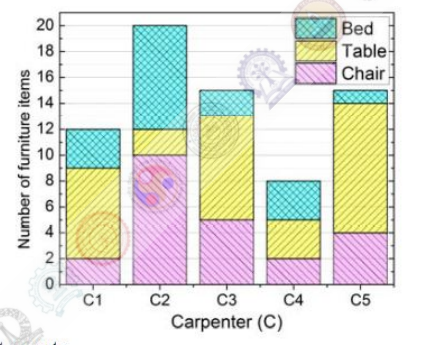
\includegraphics[width=0.5\textwidth]{figures/10.png}
\end{center}

Consider the following statements.

i. The number of beds made by carpenter C2 is exactly the same as the number of tables made by carpenter C3.
ii. The total number of chairs made by all carpenters is less than the total number of tables.

Which one of the following is true?
\begin{enumerate}
    \item[(A)] Only i  
    \item[(B)] Only ii  
    \item[(C)] Both i and ii  
    \item[(D)] Neither i nor ii  
\end{enumerate}
\vspace{0.5cm}

% Technical Section
\section*{Technical Section}

\questiona{Which one of the following plots represents the relationship \( xy = c \), where \( c \) is a positive constant}{1}
\begin{center}
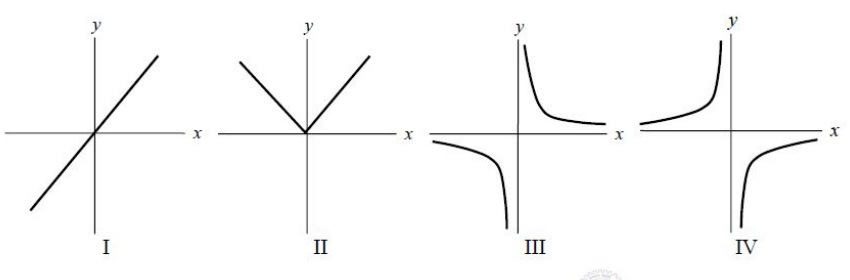
\includegraphics[width=0.8\textwidth]{figures/1.png}
\end{center}
\begin{enumerate}
    \item[(A)] I  
    \item[(B)] II  
    \item[(C)] III  
    \item[(D)] IV  
\end{enumerate}
\vspace{0.5cm}

\questiona{\( F(y) \) and \( f(y) \) are the probability distribution function and density function respectively of a continuous variable \( Y \) in the interval \((0, \infty)\). Which one of the following is TRUE?}{2}
\begin{enumerate}
    \item[(A)] \( F(y) = \int_{y}^{\infty} f(x) dx \)  
    \item[(B)] \( F(y) = \int_{0}^{y} f(x) dx \)  
    \item[(C)] \( F(y) = \frac{df(y)}{dy} \)  
    \item[(D)] \( F(y) = 1 - f(y) \)  
\end{enumerate}
\vspace{0.5cm}

\questiona{The position vector of a moving particle is given by \( \vec{r}(t) = t^3\hat{i} + t\hat{j} + t^2\hat{k} \). The acceleration of the particle in the direction of the motion is}{3}
\begin{enumerate}
    \item[(A)] 0  
    \item[(B)] \( 60\hat{i} + 2\hat{k} \)  
    \item[(C)] \( 6t\hat{i} + 4\hat{j} + 2\hat{k} \)  
    \item[(D)] \( 6t\hat{i} + 2\hat{k} \)  
\end{enumerate}
\vspace{0.5cm}

\questiona{The value of \(\lim_{x \to \infty} \left( \frac{x^2 + 2x - 1}{2x^2 - 3x - 2} \right)^{\frac{2x + 1}{2x - 1}} \)}{4}
\begin{enumerate}
    \item[(A)] \(\frac{1}{2}\)  
    \item[(B)] \(\frac{3}{2}\)  
    \item[(C)] 1  
    \item[(D)] 0  
\end{enumerate}
\vspace{0.5cm}

\questiona{Components of a 2-D stress tensor in Cartesian coordinate are \(\sigma_{xx} = 5.0 \, \text{MPa}, \, \sigma_{yy} = -10.0 \, \text{MPa}\), and \(\tau_{xy} = 2.0 \, \text{MPa}\). The traction vector (\(\vec{T}\)) in MPa acting on a plane having outward normal \(\hat{n} = \frac{\sqrt{3}}{2} \hat{i} - \frac{1}{2} \hat{j}\) is}{5}
\begin{enumerate}
    \item[(A)] \(\vec{T} = 3.33\hat{i} - 6.73\hat{j}\)  
    \item[(B)] \(\vec{T} = 3.33\hat{i} + 6.73\hat{j}\)  
    \item[(C)] \(\vec{T} = 1.73\hat{i} - 6.73\hat{j}\)  
    \item[(D)] \(\vec{T} = 1.73\hat{i} + 6.73\hat{j}\)  
\end{enumerate}
\vspace{0.5cm}

\questiona{If only two members form a truss joint and no external load or support reaction is applied to the joint, the members}{6}
\begin{enumerate}
    \item[(A)] have infinite force  
    \item[(B)] have equal but opposite force  
    \item[(C)] are zero-force members  
    \item[(D)] have unequal forces  
\end{enumerate}
\vspace{0.5cm}

\questiona{A multi-point borehole extensometer is used to monitor}{7}
\begin{enumerate}
    \item[(A)] convergence between the roof and the floor  
    \item[(B)] strain between fixed points along a borehole  
    \item[(C)] strain between the anchor point and the reference point on the surface  
    \item[(D)] changing distances between fixed points along a borehole  
\end{enumerate}
\vspace{0.5cm}

\questiona{The failure load of a point load test specimen having diameter 45 mm is 6000 N. The uncorrected point load index in MPa is \_\_\_\_\_.}{8}
\vspace{0.5cm}

\questiona{The beam shown in the figure is hinged at one end and rested on a roller at the other end. The free body diagram of the system is}{12}
\begin{center}
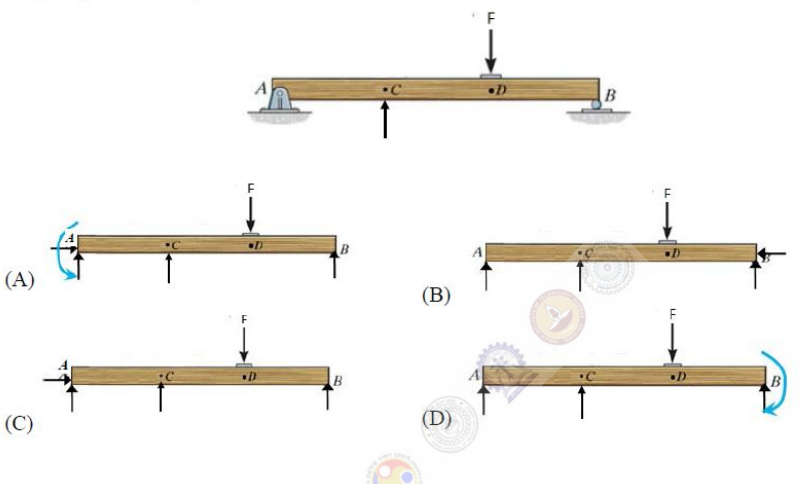
\includegraphics[width=0.9\textwidth]{figures/9.png}
\end{center}
\vspace{0.5cm}

\questiona{Minerals A and B are produced from a deposit. Minerals A and B will be called coproducts if}{10}
\begin{enumerate}
    \item[(A)] economies of mining depends upon the extraction od either mineral A or B  
    \item[(B)] economics of mining depends upon the extraction of both the minerals A and B  
    \item[(C)] mineral B is produced economically and mineral A is an additional benefit  
    \item[(D)] minerals A and B are produced in equal quantity 
\end{enumerate}
\vspace{0.5cm}

\questiona{Semi-variogram modeling is used for reserve estimation of mineral deposit by}{11}
\begin{enumerate}
    \item[(A)] polygonal method  
    \item[(B)] distance weighting method  
    \item[(C)] geostatical method  
    \item[(D)] nearest neighbour method  
\end{enumerate}
\vspace{0.5cm}

\questiona{Which one of the following does NOT belong to the direct operating cost of a mine?}{12}
\begin{enumerate}
    \item[(A)] Administrative cost  
    \item[(B)] Royalty  
    \item[(C)] Fuel cost  
    \item[(D)] Explosive cost  
\end{enumerate}
\vspace{0.5cm}

\questiona{Lane's algorithm is applied to determine}{13}
\begin{enumerate}
    \item[(A)] mill cut-off grade  
    \item[(B)] mine production rate  
    \item[(C)] operating cost  
    \item[(D)] ultimate pit  
\end{enumerate}
\vspace{0.5cm}

\questiona{In an underground coal mine a driller, wearing personal protective equipment, was going to workplace along the travelling roadway. A piece of rock fell down from the roof and hit the person on head causing serious injury. The cause of accident is}{14}
\begin{enumerate}
    \item[(A)] unsafe act of the driller  
    \item[(B)] job stress  
    \item[(C)] unsafe act and unsafe condition  
    \item[(D)] unsafe condition  
\end{enumerate}
\vspace{0.5cm}

\questiona{In a PERT network, the "time estimates" of an activity are the following: Optimistic time - 2 days, Most likely time - 4 days, and Pessimistic time - 12 days. The expected time and standard deviation of the activity in days are respectively}{15}
\begin{enumerate}
    \item[(A)] 6.0 and 2.78  
    \item[(B)] 5.0 and 1.66  
    \item[(C)] 6.0 and 1.66  
    \item[(D)] 5.0 and 2.78  
\end{enumerate}
\vspace{0.5cm}

\questiona{The magnetic bearing of a line is \( 65^\circ 30' \). If the declination is \( 4^\circ 30' \, W \), the true bearing of the line in degrees is \_\_\_\_\_.}{16}
\vspace{0.5cm}

\questiona{A vertical photograph of a 40 m high hill is taken from 4.4 km height. If the focal length of the camera is 15 cm, the scale of the photograph is \_\_\_\_\_.}{17}
\begin{enumerate}
    \item[(A)] 1 in 29067  
    \item[(B)] 1 in 7267  
    \item[(C)] 1 in 29050  
    \item[(D)] 1 in 9688  
\end{enumerate}
\vspace{0.5cm}

\questiona{The operating conditions of a rotary rock drill are: applied thrust: 6.75 kN, revolution: 180 rpm, and penetration rate: 0.15 m/min. The work done per revolution in N-m is \_\_\_\_\_.}{18}
\vspace{0.5cm}

\questiona{The Absolute amount of energy and density of a booster and ANFO are given below.}{19}

\begin{center}
\begin{tabular}{|l|c|c|}
\hline
Explosive type & Energy (cal/g) & Density (g/cc) \\
\hline
Booster & 680 & 1.25 \\
ANFO & 912 & 0.81 \\
\hline
\end{tabular}
\end{center}

The Relative bulk strength of booster is \_\_\_\_\_.
\vspace{0.5cm}

\questiona{A deeply seated ore body dips at 70° having an average width of 60 m. The ore body, hanging wall, and footwall are competent. The suitable stoping method for this ore body is}{20}
\begin{enumerate}
    \item[(A)] Post pillar cut and fill  
    \item[(B)] Shrinkage stoping  
    \item[(C)] Transverse sublevel caving  
    \item[(D)] Transverse sublevel open stoping  
\end{enumerate}
\vspace{0.5cm}

\questiona{The results of the crossing point temperature experiments for coal A and B are shown in the figure.}{21}

\begin{center}
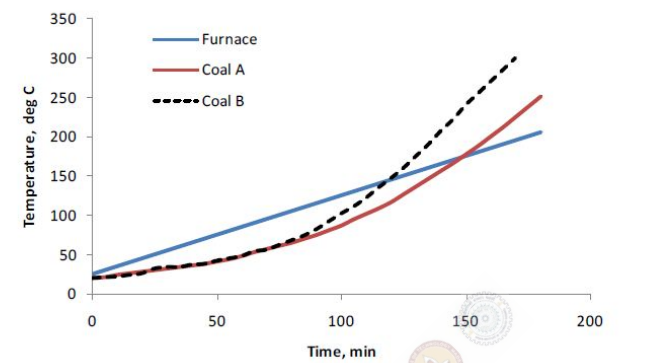
\includegraphics[width=0.5\textwidth]{figures/21.png}
\end{center}

The correct interpretation of the plot is that
\begin{enumerate}
    \item[(A)] coal A is more prone to spontaneous heating than coal B  
    \item[(B)] coal B is more prone to spontaneous heating than coal A  
    \item[(C)] coal A is more prone to coal dust explosion than coal B  
    \item[(D)] coal B is more prone to coal dust explosion than coal A  
\end{enumerate}
\vspace{0.5cm}

\questiona{The "yellow boy" formed due to acid mine drainage mainly consists of}{22}
\begin{enumerate}
    \item[(A)] Ferrous hydroxide  
    \item[(B)] Ferrous sulfate  
    \item[(C)] Ferric hydroxide  
    \item[(D)] Ferric sulfate  
\end{enumerate}
\vspace{0.5cm}

\questiona{A double ended ranging drum shearer is employed in a longwall mine of face length 150 m. The mining height is 3.5 m and depth of the web cut is 0.76 m. The cycle time for unidirectional cutting is 40 min. Considering bulk density of the coal to be \(1.4 \, \text{t/m}^3\), hourly production from the face in tonne is \_\_\_\_\_.}{23}
\vspace{0.5cm}

\questiona{The strength of a stranded wire rope is proportional to}{24}
\begin{enumerate}
    \item[(A)] the diameter of the rope  
    \item[(B)] square of the diameter of the rope  
    \item[(C)] square root of the diameter of the rope  
    \item[(D)] inverse of the diameter of the rope  
\end{enumerate}
\vspace{0.5cm}

\questiona{A 20 m thick and 30 m wide confined aquifer has two monitoring wells spaced 500 m apart along the direction of groundwater flow. The difference in water level between the wells is 2 m. The hydraulic conductivity is 50 m/day. The rate of flow in \( m^3/\text{day} \) is}{25}
\begin{enumerate}
    \item[(A)] 4  
    \item[(B)] 12  
    \item[(C)] 40  
    \item[(D)] 120  
\end{enumerate}
\vspace{0.5cm}

\questionb{The \( y \) intercept of the tangent of curve \( y = x^3 - x^2 + x - 1 \) at \( x = 1 \) is \_\_\_\_\_.}{26}
\vspace{0.5cm}

\questionb{A rectangle has two of its corners on the \( x \) axis and the other two on the parabola \( y = 12 - x^2 \). The largest area of the rectangle is \_\_\_\_\_.}{27}
\vspace{0.5cm}

\questionb{The area of cross-section (\(x\)) of four rock samples and the respective applied loads (\(y\)) at failure under uniaxial loading are given below:}{28}

\[
\begin{array}{c|cccc}
x \, (\text{cm}^2) & 7 & 10 & 13 & 16 \\
\hline
y \, (\text{kN}) & 35 & 45 & 60 & 80 \\
\end{array}
\]

If the best fit line \( y = 4.88x \) represents the above data, the coefficient of determination (\( R^2 \)) of the best fit line is \_\_\_\_\_.
\vspace{0.5cm}

\questionb{The following readings refer to a reciprocal leveling at staff stations A and B respectively:}{29}

\begin{center}
\begin{tabular}{|c|c|c|l|}
\hline
Instrument station & Staff reading (m) & Remarks \\
 & A & B & \\
\hline
P & 1.725 & 2.835 & RL of A = 125.0 m \\
Q & 0.835 & 1.545 & \\
\hline
\end{tabular}
\end{center}

The reduced level (RL) of staff station B in m is \_\_\_\_\_.
\vspace{0.5cm}

\questionb{The areas within the contour lines of a proposed site for an overburden dump are as follows:}{30}

\begin{center}
\begin{tabular}{|c|c|}
\hline
Contour RL (m) & Area (m\(^2\)) \\
\hline
195 & 3054 \\
180 & 3025 \\
165 & 2095 \\
150 & 2008 \\
135 & 2000 \\
120 & 1992 \\
\hline
\end{tabular}
\end{center}

The total volume of overburden in cubic meter that could be dumped within the 120 m and 195 m contour levels is \_\_\_\_\_.
\vspace{0.5cm}

\questionb{Total ore mined from a sub-level open stope of a copper deposit is measured to be 100000 tonne. The ore recovery and ore dilution during stoping are 90\% and 20\% respectively. The in situ Cu grade of the ore in the stope is 0.65\%. The selling price of copper is Rs. 400/kg of metal. Ignoring any other metal losses in the downstream process of the ore, the revenue generated by selling the ore in Crores of rupees is \_\_\_\_\_.}{31}
\vspace{0.5cm}

\questionb{The block grade model of an ore deposit is shown in the figure below. The relationship between block value per tonne (\(B_v\)) in rupees and the block grade in percentage (\(x\)) is given below:}{32}

\[
B_v = -38500 + 700 \times x, \quad \text{for } x \geq 55\% \\
= -300, \quad \text{otherwise}
\]

\begin{center}
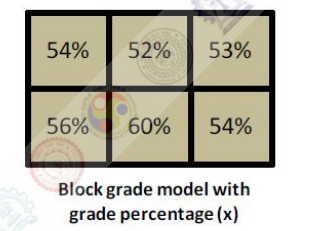
\includegraphics[width=0.5\textwidth]{figures/32.png}
\end{center}

If each square block contains 1000 tonne of material and the overall pit slope angle is \(45^\circ\), the total value of the pit determined by the floating cone algorithm in Lakhs of rupees is \_\_\_\_\_.
\vspace{0.5cm}

\questionb{A mine is being developed by bord and pillar method with a gallery size of \(4.8 \, \text{m} \times 2.4 \, \text{m}\). The mine operates in 3 shifts per day and 6 faces are blasted per shift. The average pull per round of blast is \(1.2 \, \text{m}\) and the bulk density of coal is \(1.4 \, \text{t/m}^3\). If the OMS is \(2.5\), then the average manpower deployed in the development section per shift is \_\_\_\_\_.}{33}
\vspace{0.5cm}

\questionb{Consider the following linear programming problem:}{34}

Maximize  
\[ Z = 6X + 10Y \]  
Subject to  
\[ X \leq 4 \]  
\[ Y \leq 6 \]  
\[ 3X + 2Y \leq 18 \]  
\[ X \geq 0, \, Y \geq 0 \]

The maximum value of the objective function is \_\_\_\_\_.
\vspace{0.5cm}

\questionb{A mining company having three mines A, B and C supplies coal to three power plants P, Q and R located close to the mines. The daily production capacities of the three mines in tonnes are 700, 1200, and 1100 respectively. The daily requirements at the power plants in tonnes are 1000, 1000, and 1000 respectively. The transportation costs in rupees per tonne is given in the matrix below:}{35}

\begin{center}
\begin{tabular}{|c|c|c|c|}
\hline
Power plant & P & Q & R \\
\hline
Mine & & & \\
A & 15 & 20 & 60 \\
B & 5 & 40 & 20 \\
C & 30 & 10 & 50 \\
\hline
\end{tabular}
\end{center}

The total cost of coal transportation in rupees from the three mines to three power plants using the least-cost method is \_\_\_\_\_.
\vspace{0.5cm}

\questionb{The series-parallel configuration of a system, consisting of 6 independent components A, B, C, D, E, and F with their individual reliability, is shown in the figure:}{36}

\begin{center}
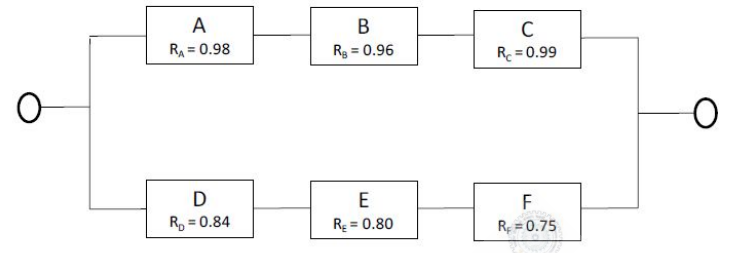
\includegraphics[width=0.8\textwidth]{figures/36.png}
\end{center}

The reliability of the system is \_\_\_\_\_.
\vspace{0.5cm}

\questionb{500 coal miners were randomly selected from an underground coal mine. It was found that 50 workers experienced an injury in the year 2014. The distribution of injury based on younger age group (\( age \leq 40 \) years) and older age group (\( age > 40 \) years) generated the following cross classification table.}{37}

\begin{center}
\begin{tabular}{|c|c|c|c|}
\hline
Age group & Number of workers & Row total \\
 & Injured & Non-injured & \\
\hline
Younger age group & 20 & 130 & 150 \\
Older age group & 30 & 320 & 350 \\
Column total & 50 & 450 & 500 \\
\hline
\end{tabular}
\end{center}

The odds of injury for the younger age group compared to the older age group is \_\_\_\_\_.
\vspace{0.5cm}

\questionb{A bord and pillar panel is being planned at a depth of 300 m. The dimension of square pillar is 35 m centre-to-centre. The average unit weight of the overburden rock is 25 kN/m\(^3\). If the strength of the pillar is 14.0 MPa, the gallery width in m for a safety factor of 1.3 is \_\_\_\_\_.}{38}
\vspace{0.5cm}

\questionb{A sandstone sample having 15\% moisture content and volume of 75 cm\(^3\) weighs 180 g. If the grain density is 2.6 g/cm\(^3\), porosity of the sample in \% is \_\_\_\_\_.}{39}
\vspace{0.5cm}

\questionb{Let \(\sigma_1\) and \(\sigma_3\) are major and minor principal stresses respectively. The equation \(\sigma_1 = f(\sigma_3)\) denotes the failure envelop of a rock as shown in the figure. Match the zones (P, Q, R and S) with the legend code.}{40}

\begin{center}
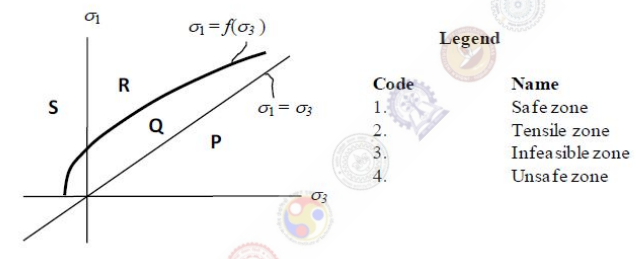
\includegraphics[width=0.7\textwidth]{figures/40.png}
\end{center}

\begin{enumerate}
    \item[(A)] \(P\)-1, \(Q\)-2, \(R\)-4, \(S\)-3
    \item[(B)] \(P\)-3, \(Q\)-1, \(R\)-4, \(S\)-2
    \item[(C)] \(P\)-3, \(Q\)-1, \(R\)-2, \(S\)-4
    \item[(D)] \(P\)-1, \(Q\)-4, \(R\)-3, \(S\)-2
\end{enumerate}

\vspace{0.5cm}

\questionb{A blasted muck of mass \( m \) is being lifted from a shaft of diameter \( d \) by an arrangement of two pulleys as shown in the figure. Ignoring friction in the pulleys, as the height \( h \) decreases, tension in the ropes}{41}
\begin{enumerate}
    \item[(A)] increases  
    \item[(B)] decreases  
    \item[(C)] remains constant  
    \item[(D)] increases until \( h > d \), then decreases  
\end{enumerate}
\vspace{0.5cm}

\begin{center}
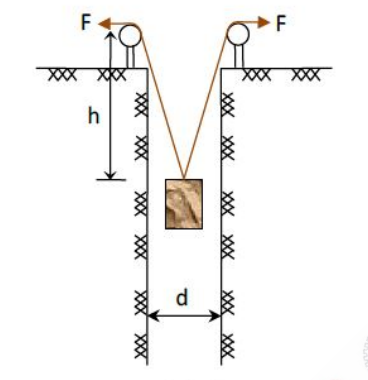
\includegraphics[width=0.5\textwidth]{figures/41.png}
\end{center}

\questionb{The longitudinal section of a slope is given in the figure. Match the different labeled slope features (P, Q, R, S, and T) with their corresponding nomenclatures.}{42}

\begin{center}
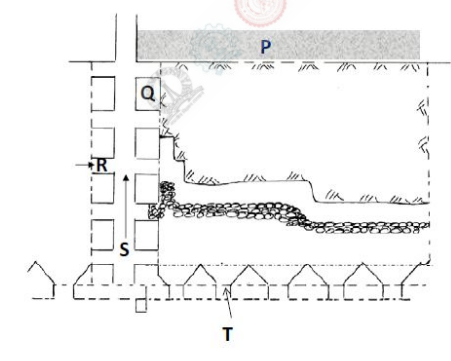
\includegraphics[width=0.7\textwidth]{figures/42.png}
\end{center}

\begin{center}
\begin{tabular}{|c|l|}
\hline
\textbf{Code} & \textbf{Name} \\
\hline
1 & Box hole \\
2 & Raise \\
3 & Crown Pillar \\
4 & Access drift \\
5 & Bip Pillar \\
\hline
\end{tabular}
\end{center}

\begin{enumerate}
    \item[(A)] P-2, Q-3, R-1, S-5, T-4  
    \item[(B)] P-5, Q-1, R-2, S-3, T-4  
    \item[(C)] P-3, Q-5, R-4, S-2, T-1  
    \item[(D)] P-1, Q-5, R-3, S-4, T-2  
\end{enumerate}
\vspace{0.5cm}

\questionb{To break a volume of 300000 cubic meter of overburden per month in an open cast mine, the number of blast hole drills required for the following data is \_\_\_\_\_}{43}

\begin{tabular}{ll}
Spacing and burden of blast holes: & 6.0 m $\times$ 4.0 m \\
Hours scheduled per shift: & 5 \\
Number of shifts per day: & 2 \\
Weeks per month: & 4 \\
Drilling days per week: & 5 \\
Drilling rate: & 30.67 m/h \\
\end{tabular}
\vspace{0.5cm}

\questionb{Two inclined coal seams with their accesses are shown in the figure. Match the labeled access (P, Q, R, S) with their corresponding names.}{44}

\begin{center}
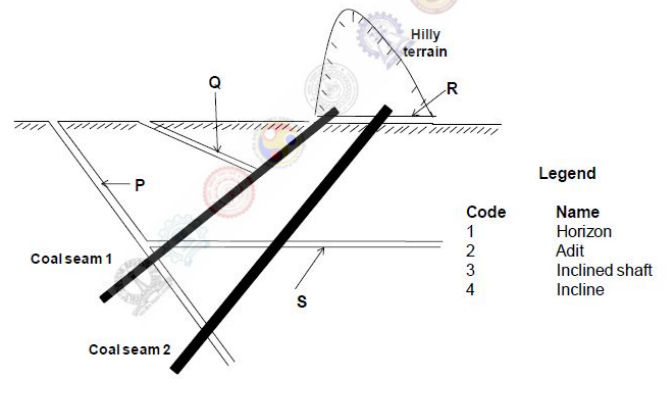
\includegraphics[width=0.8\textwidth]{figures/44.png}
\end{center}

\begin{enumerate}
    \item[(A)] P-4, Q-3, R-1, S-2
    \item[(B)] P-4, Q-3, R-2, S-1
    \item[(C)] P-3, Q-4, S-2, R-1
    \item[(D)] P-3, Q-4, R-2, S-1
\end{enumerate}
\vspace{0.5cm}

\questionb{Ground reaction curve (GRC) of a tunnel roof under hydrostatic stress field is given by $p_g = 10 - 0.75u$, where $p_g$ is the required support pressure in MPa and $u$ is radial displacement in mm. A uniform support is installed at the boundary of the tunnel providing support reaction (SR) as $p_s = 1.5u - 3.0$, for $u \geq 2$ mm. Considering GRC = SR, the support pressure in MPa is \_\_\_\_\_.}{45}
\vspace{0.5cm}

\questionb{If the rank of the following matrix is less than 3, the values of \( x \) are}{46}

\[
A = \begin{bmatrix} 
1 & x & x \\ 
x & 1 & x \\ 
x & x & 1 
\end{bmatrix}
\]

\begin{enumerate}
    \item[(A)] 1, \(-1/2\)  
    \item[(B)] 1, \(1/2\)  
    \item[(C)] 2, \(-1/4\)  
    \item[(D)] 2, \(-3/4\)
\end{enumerate}
\vspace{0.5cm}

\questionb{The discharge rate of a water pump is 0.25 m\(^3\)/s. The diameter of the discharge and suction nozzles are 300 and 350 mm respectively. The measured pressure at the discharge end located 0.25 m above the centerline of the impeller is 150 kN/m\(^2\) and the pressure at the suction gage located at the centre line of the impeller is 20 kN/m\(^2\). Specific weight of water is 9810 N/m\(^3\). The total dynamic head for the above installation in m is \_\_\_\_\_.}{47}
\vspace{0.5cm}

\questionb{In a mine, 200 and 250 persons are deployed in the Panels A and B (shown in figure) respectively in the largest shift. The panels produce 400 and 500 tonne/day respectively. The resistances of panels A and B are 0.3 \( \text{Ns}^2\text{m}^{-8} \) and 0.4 \( \text{Ns}^2\text{m}^{-8} \) respectively and the combined resistance of shaft and trunk airways is 0.5 \( \text{Ns}^2\text{m}^{-8} \). The operating static pressure of the fan in Pa to provide the minimum air quantities in the panels as per CMR 1957 is \_\_\_\_\_.}{48}

\begin{center}
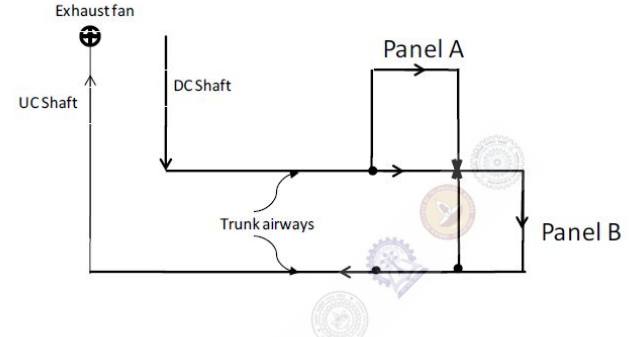
\includegraphics[width=0.5\textwidth]{figures/48.png}
\end{center}
\vspace{0.5cm}

\questionb{In an auxiliary ventilation system, a fan is installed inside a 100 m long and 600 mm diameter duct to ventilate a blind heading face. The frictional coefficient of the duct is 0.0066 \( \text{Ns}^2\text{m}^{-4} \) and the static pressure characteristic of the fan is represented by:}{49}

\[
P_s = 5Q^2 - 250Q + 1000
\]

where, \( P_s \) is in Pa and Q is in \( \text{m}^3/\text{s} \). The quantity of air delivered by the fan in \( \text{m}^3/\text{s} \) is \_\_\_\_\_.
\vspace{0.5cm}

\questionb{A stream flowing at 15 \( \text{m}^3/\text{s} \) has a tributary feeding into it with a flow rate of 7 \( \text{m}^3/\text{s} \). The concentrations of chloride at the upstream of the junction and that of the tributary are 30 mg/L, and 50 mg/L respectively. Treating chloride as conservative substance and assuming complete mixing of two streams, the concentration of chloride in mg/L at the downstream is \_\_\_\_\_.}{50}
\vspace{0.5cm}

\questionb{A sample of mine water has 100 mg/L of \( Ca^{2+} \) and 10 mg/L of \( Mg^{2+} \). The equivalent weights of \( Ca^{2+} \) and \( Mg^{2+} \) are 20 mg/meq and 12.2 mg/meq respectively. The hardness of mine water in unit of mg/L as CaCO\(_3\) is \_\_\_\_\_.}{51}
\vspace{0.5cm}

\questionb{A 1.1 m wide belt conveyor carries materials of bulk density 1.35 t/m\(^3\) at a speed of 1.75 m/s. The average cross-sectional area of material is equal to \( w^2 / 11 \), where \( w \) is the width of the belt in m. The carrying capacity of the conveyor in t/h is \_\_\_\_\_.}{52}
\vspace{0.5cm}

\questionb{In a book of 600 pages, there are 60 typographical errors. Assuming Poisson distribution for the number of errors per page, the probability of no errors in randomly chosen 4 pages is \_\_\_\_\_.}{53}
\vspace{0.5cm}

\questionb{Match the special methods of shaft sinking with rock mass conditions and scope of application.}{54}

\begin{center}
\begin{tabular}{|l|l|l|}
\hline
Special methods & Rock mass condition & Scope of application \\
\hline
A. Shaft boring & P. Loose ground without intrusion of hard rocks or boulders & 1. Any depth \\
B. Cement grouting & Q. Highly jointed rock filled with water & 2. Up to 30 m from surface \\
C. Caisson method & R. All types of water bearing rocks & 3. Up to 1000 m \\
D. Freezing & S. Moderately strong rocks & 4. Less than 600 m from surface \\
\hline
\end{tabular}
\end{center}

\begin{enumerate}
    \item[(A)] A-S-3, B-R-2, C-Q-1, D-P-4  
    \item[(B)] A-P-2, B-Q-1, C-S-4, D-R-3  
    \item[(C)] A-R-3, B-P-1, C-S-2, D-Q-4  
    \item[(D)] A-S-4, B-Q-1, C-P-2, D-R-3  
\end{enumerate}
\vspace{0.5cm}

\questionb{A wheel of radius 0.5 m rotates under a moment of 2000 N-m as shown in the figure. A block brake is used to stop the wheel. If the coefficient of static friction between the wheel and the block brake is 0.3, the smallest force of P in N required to stop the wheel is \_\_\_\_\_.}{55}

\begin{center}
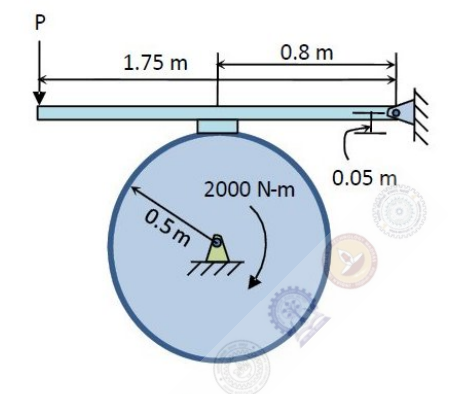
\includegraphics[width=0.5\textwidth]{figures/55.png}
\end{center}
\vspace{0.5cm}

\vspace{5cm}
\begin{center}
\textbf{END OF THE QUESTION PAPER} \\
\rule{\textwidth}{0.5pt}
\end{center}

\end{document}


\end{document}